\documentclass[letterpaper]{article}
\let\oldvec\vec
\usepackage[bottom=0.7in, left=.5in, right=1in, top=.7in]{geometry}
\usepackage[utf8]{inputenc}
\usepackage[T1]{fontenc}
\usepackage[english]{babel}
\usepackage{fancyhdr}
\usepackage{graphicx}
\usepackage{caption}
%\captionsetup{justification   = raggedright,
%	singlelinecheck = false}
\usepackage{physics}
\usepackage{amsfonts}
\usepackage{amsmath, amssymb}
\usepackage[breaklinks=true, hidelinks=true]{hyperref}
\usepackage[nottoc, numbib]{tocbibind}
\usepackage[
sorting=ynt
]{biblatex}
\addbibresource{bibliography.bib}

\pagestyle{fancy}
\pagenumbering{arabic}
\rhead{Angelica Urbanelli S271114}
\lhead{Data Spaces, a.y. 2020/2021}

\begin{document}
	\title{Tesina}
	\author{Angelica Urbanelli S271114}
	\date{Data Spaces, a.y. 2020/2021}
	\maketitle
	
	\tableofcontents
	
	\newpage 
	\section{Introduction}
	-spiegare il problema
	importanza di distinguere buoni e cattivi pagatori
	statistiche?
	
	-interpretabilità?
	-falsi buoni peggio di falsi cattivi
	
	
	-tutto il codice si trova nella repo github xx
	-per navigarlo e browsing all images usare il link xx di jupyternotebook
	
	\section{Dataset description}
	\subsection{History}
	The dataset used comes from the UCI Machine Learning Repository \cite{uci}, under the name "South German Credit (UPDATE) Data Set" \cite{dataset}. \\
	Ulrike Grömping, professor at the Beuth University in Berlin, in her paper \cite{gromping} provides the history of this dataset, her considerations about the data and corrections on the code table.\\
	Basically, the data come from a large regional bank in the southern Germany that have been collected from 1973 to 1975, and have been originally provided to UCI in 1994 by Professor Dr. Hans Hofmann from Hamburg University \cite{hofmann} as part of a group of datasets in the context of the EU Statelog Project.\\
	Because of many inconsistencies, found while trying to interpret the final results of her experiments, Grömping decided to research the story of this data, that she found in the German literature together with the same dataset with some differences. These informations helped her to fix the code table (a file that explains the encoding of categorical variables) of this dataset and consequently to provide the correct one (now attached in the .zip downloadable from UCI). \\ 
	%TODO: write the inconsistencies? 
	Grömping also explained that it was worth it because, although the dataset contains very old data, it is widely used in many researches in the domain of interpretable machine learning, indeed there are various R packages that include this data. In addition, it \emph{is one of the few data sets on credit scoring that has a meaning attached to variables and their levels}, which is a very important feature when using this kind of data to do experiments whose interpretability is a key point of research.  \\
	
	\subsection{General structure}
	The dataset contains 1000 samples, each one characterized by 20 features and classified as \texttt{good} or \texttt{bad credit risk}, in particular there are 700 good ones and 300 bad ones [Figure \ref{fig:1}].  Customers with good credits perfectly complied with the conditions of the contract, while customers with bad credits did not comply with the contract as required.\\ As reported in the aforementioned paper \cite{gromping}, the actual percentage of bad credits was around 5\%, and examples of bad credit risk have been heavily oversampled. 
	
	\begin{figure}[h]
		\centering
		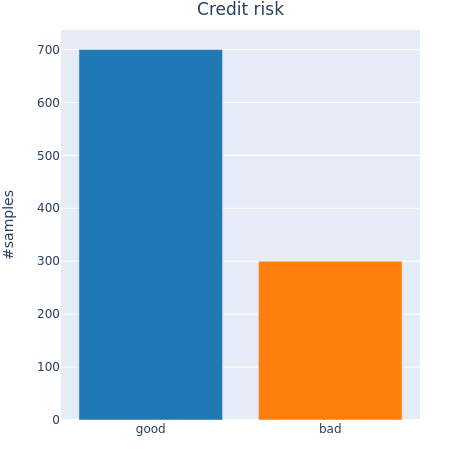
\includegraphics[width=.35\textwidth]{images/class.png}
		\captionof{figure}{\texttt{good} and \texttt{bad} credit risk distribution}
		\label{fig:1}
		
	\end{figure}
	
	\subsection{Features description}
	Among the 20 features, there are 3 numerical discrete variables:
	\begin{itemize}
		\item \textbf{duration}: credit duration in months
		\item \textbf{amount}: credit amount in DM\footnote{stands for Deutsche Mark, was the official currency of West Germany from 1948 until 1990 and later the unified Germany from 1990 until 2002 \cite{dm}}; original values are not available, the ones present in the dataset are the result of an unknown monotonic transformation
		\item \textbf{age}: age of the debtor in years
	\end{itemize}
	10 ordinal variables; most of theme were numerical ones on which binning has been applied, that means that they have been aggregated into a fixed number of intervals, so that they can be treated as ordinal features:
	\begin{itemize}
		\item \textbf{employment\_duration}:  duration of debtor’s employment with current employer (unemployed; < 1 year ; $\geq$ 1 and < 4 years; $\geq$ 4 and < 7 years; $\geq$ 7 years)
		\item \textbf{installment\_rate}: credit installments expressed as a percentage of debtor’s disposable income ( $\geq$ 35; $\geq$ 25 and < 35; $\geq$ 20 and < 25; < 20); it is the only ordinal feature expressed in a decreasing order
		\item \textbf{present\_residence}: from how many years the debtor lives in the present residence (< 1 year ; $\geq$ 1 and < 4 years; $\geq$ 4 and < 7 years; $\geq$ 7 years)
		\item \textbf{number\_credits}:  number of credits including the current one the debtor has (or had) at this bank (1; 2 or 3; 4 or 5; $\geq$ 6)
		\item \textbf{people\_liable}: number of people who financially depend on the debtor (i.e., are entitled to maintenance) (from 0 to 2; 3 or more)
		\item \textbf{status\footnotemark}: status of the debtor’s checking account with the bank in DM (no checking account; < 0; 0 $\leq$ ... < 200; $\geq$ 200 / salary for at least 1 year)
		\item \textbf{savings\footnotemark[\value{footnote}]}: debtor’s savings in DM (unknown/no savings account; <  100; 100 $\leq$ ... <  500; 500 $\leq$ ... < 1000; $\leq$ 1000 )
		\item \textbf{credit\_history\footnotemark[\value{footnote}]}:  history of compliance with previous or concurrent credit contracts (delay in paying off in the past; critical account/other credits elsewhere; no credits taken/all credits paid back duly; existing credits paid back duly till now; all credits at this bank paid back duly )
		\item \textbf{job}: quality of debtor’s job (unemployed/unskilled - non-resident; unskilled - resident; skilled employee/official; manager/self-employed/highly qualified employee)
		\item \textbf{property}:  the debtor’s most valuable property, i.e. the highest possible code is used ( unknown / no property; car or other [savings don't fall into this category]; building society savings agreement (mortgage)/life insurance; real estate )
	\end{itemize}
	\footnotetext{Those are considered as categorical by Grömping \cite{gromping}, but in my opinion their labels can be ranked and also considering that to properly manage categorical features an encoding have to be done, thus likely this brings to a huge number of features. Possibly, the position of \emph{no checking account} in \texttt{status} feature could be discussed with a domain expert.}
	7 categorical variables:
	\begin{itemize}
		\item \textbf{purpose}:  purpose for which the credit is needed (others; car (new); car (used); furniture/equipment; radio/television; domestic appliances; repairs; education; vacation; retraining; business)
		\item \textbf{personal\_status\_sex}:  combined information on sex and marital status; sex cannot be recovered from the variable because male singles and female non-singles are coded with the same code; in addition, female widows are not listed in any of the categories (male divorced/separated; female non-single or male single; male married/widowed; female single)
		\item \textbf{other\_debtors}: whether there is another debtor or a guarantor for the credit (none; co-applicant; guarantor)
		\item \textbf{other\_installment\_plans}: installment plans from providers other than the credit-giving bank (bank; stores; none)
		\item \textbf{housing}:  type of housing the debtor lives in (for free; rent; own)
		\item \textbf{telephone}:  whether there is a telephone landline registered on the debtor’s name; of course this variable would have no meaning nowadays, but this data come from 1970s (yes; no)
		\item \textbf{foreign\_worker}: whether the debtor is a foreign worker (yes; no)
	\end{itemize}	
	\section{Dataset Analysis}
		\begin{figure}[h]
		\centering
		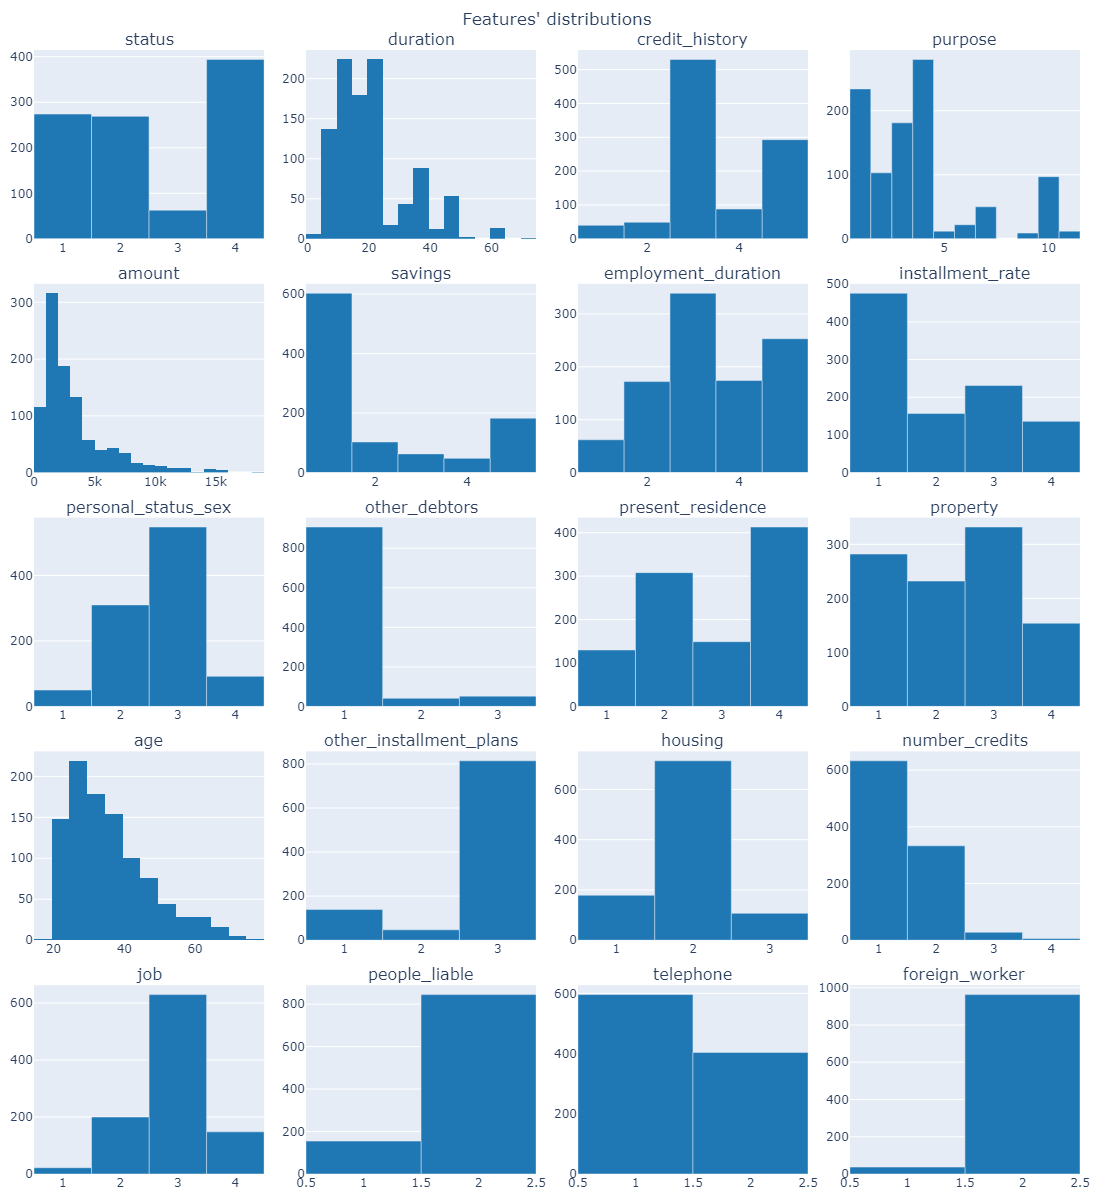
\includegraphics[width=.8\textwidth]{images/distributions.png}
		\captionof{figure}{Features' distributions}
		\label{fig:2}
	\end{figure}
	\begin{figure}[h]
		\centering
		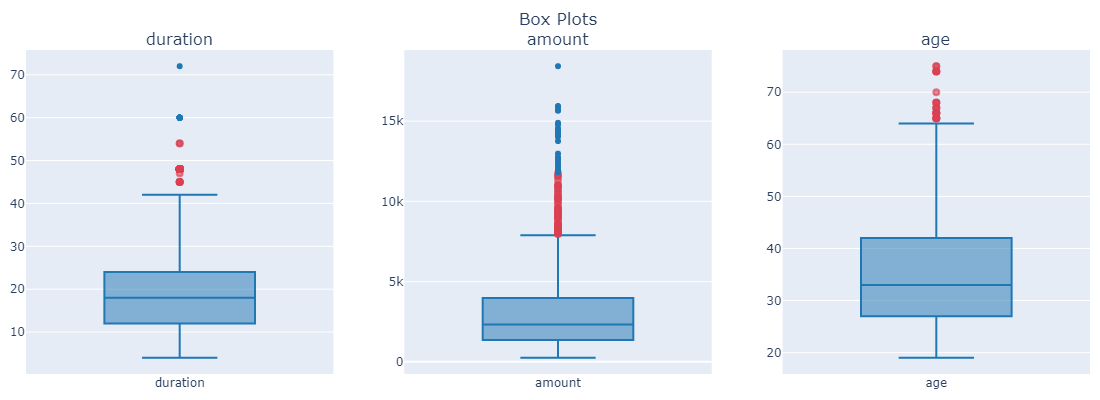
\includegraphics[width=.85\textwidth]{images/significant_boxplots.png}
		\captionof{figure}{Box Plots of \texttt{duration}, \texttt{amount} ad \texttt{age}}
		\label{fig:3}
	\end{figure}
	
	\subsection{Features' distributions} \label{features distrubution}
	Here [Figure \ref{fig:2}] the distribution of the various features can be seen. Some of them are highly imbalanced, for instance it can be noticed that almost all customers are not foreigners and have neither another debtor nor a guarantor for the credit. \\
	% TODO la documentazione meglio metterla come nota o tra parentesi inserendo l'url
	It might be interesting to take a look at the box plots of the numerical discrete features: \texttt{duration}, \texttt{amount} ad \texttt{age}  [Figure \ref{fig:3}]. Given that $Q_1$ and $Q_3$ are, respectively, the first and the third quartile, and that the interquartile range $IQR = Q_3 - Q_1$, in the chosen representation the whiskers are: the largest observed point that falls within $Q_3$ and $Q_3 + 1.5\cdot Q_3$ and the lowest observed point that falls within $Q_1$ and $Q_1 - 1.5\cdot Q_1$ \cite{boxplots_wiki}. The single points, instead, are highlighted in red if they fall within the lowest whisker and $4\cdot Q_1 - 3\cdot Q_3$ or within the highest whisker and  $4\cdot Q_3 - 3\cdot Q_1$ \cite{boxplots}, those are called \emph{suspected} outliers; while the blue points are the ones outside these ranges, thus they can be considered outliers beyond any doubt. \\
	In this case, since those plots represent the univariate distribution, those points are not considered as outliers; they will be better evaluated and managed in section \ref{outliers}.

	\subsection{Features distribution per class}
	In figure [\ref{fig:4}] and [\ref{fig:5}], the same plots of section \ref{features distrubution} are shown, highlighting the distributions separately for the two class labels. 
	\begin{figure}[h]
		\centering
		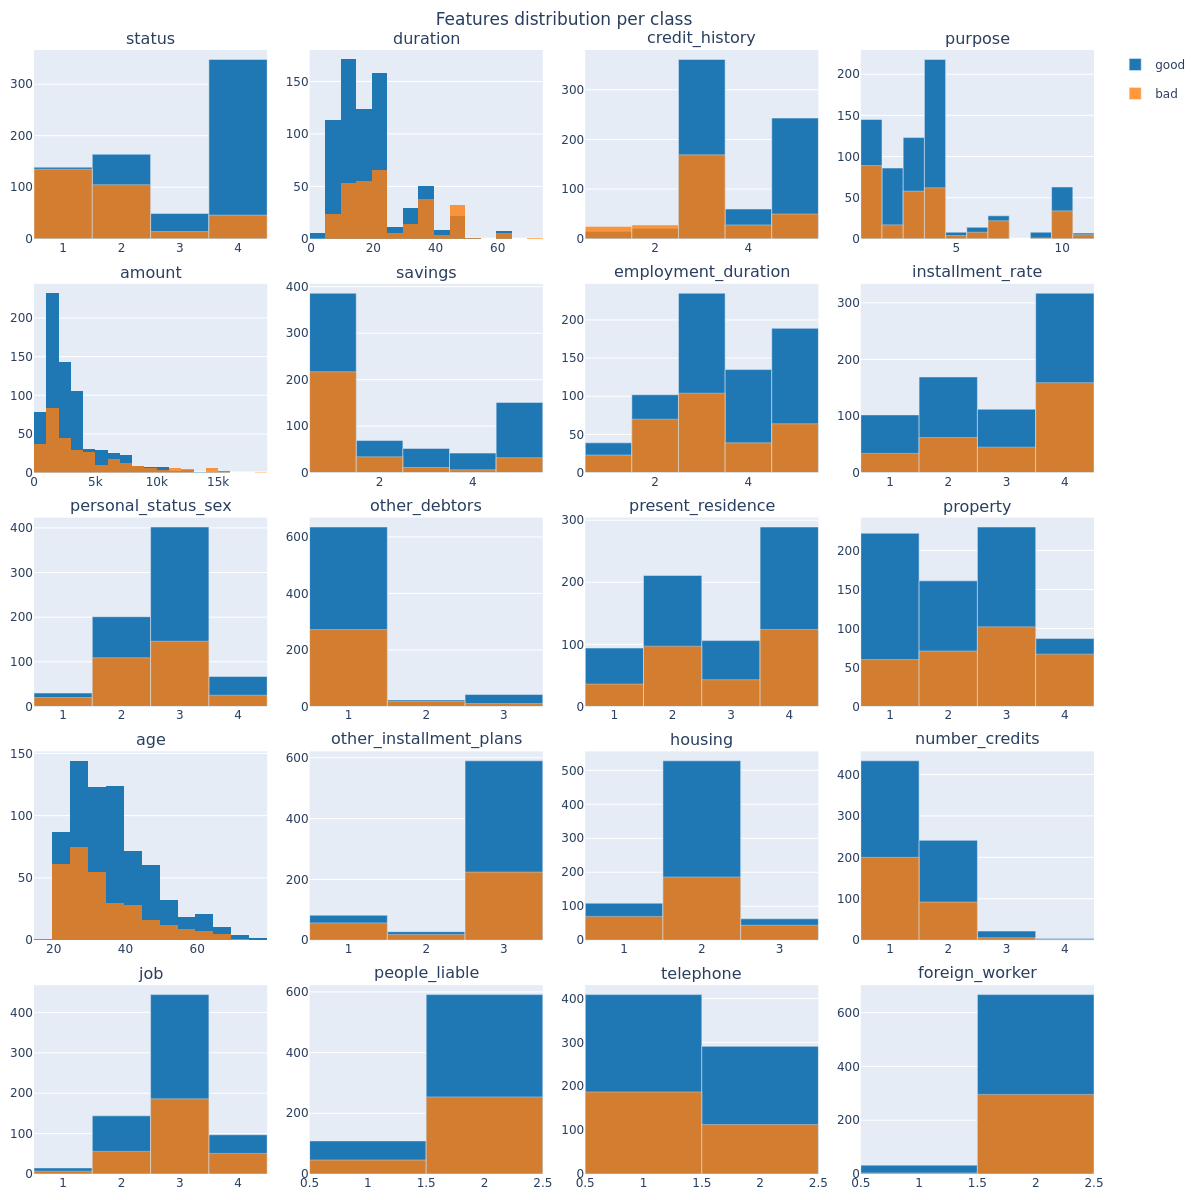
\includegraphics[width=.8\textwidth]{images/distributions_by_class.png}
		\captionof{figure}{Features' distributions per class}
		\label{fig:4}
	\end{figure}
	\begin{figure}[h]
		\centering
		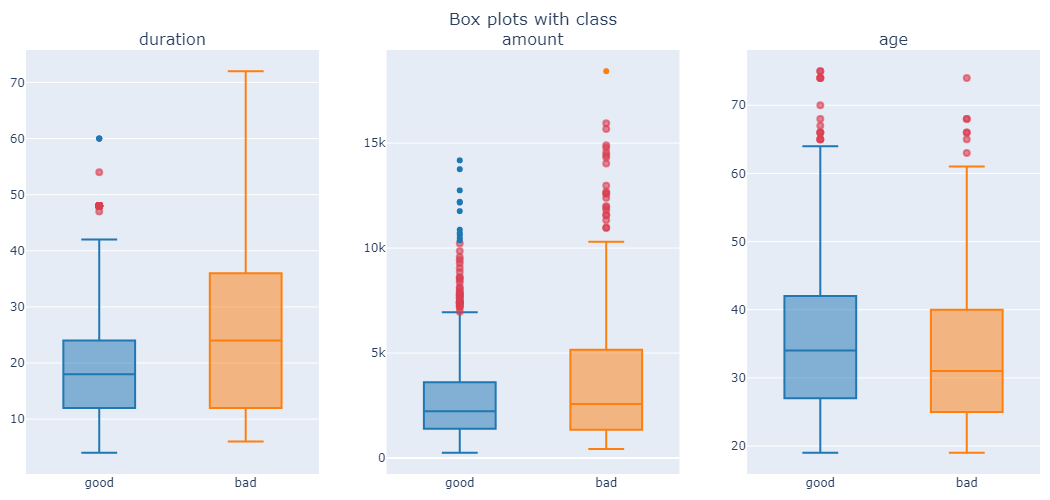
\includegraphics[width=.85\textwidth]{images/boxplots_with_classes.png}
		\captionof{figure}{Box Plots of \texttt{duration}, \texttt{amount} ad \texttt{age} divided by class}
		\label{fig:5}
	\end{figure}
	
	\section{Data preprocessing}
	\subsection{Labels encoding}
	All the features' labels are expressed as integers: both categorical and ordinal ones have been previously mapped to integers by the donor of the data, using label encoding either from 0 to N-1 (only for \textbf{purpose} and \textbf{credit\_history}) or from 1 to N (all the other variables) where N is the number of labels for a certain feature. Apparently there is no particular reason for this distinction. For what concerns class labels (\texttt{credit risk}), they have been mapped to $0$ for \texttt{bad} and $1$ for \texttt{good}. \\
	\paragraph{}In order to make variables more uniform, two small changes have been done:
	\begin{itemize}
		\item the variable \textbf{installment\_rate} is the only one among the ordinal variables having a decreasing order, so its mapping has been inverted; thus now label \texttt{1} means $< 20$, label \texttt{2} means $\geq 20$ and $< 25$ and so on;
		\item \textbf{credit\_history} and \textbf{purpose}'s mappings have been changed from $0 \rightarrow N-1$ to $1 \rightarrow N$;
		\item in this kind of classification, the \emph{positive} class is the one we are more interested in correctly classifying, in this case the \texttt{bad} creditors. By convention, the \emph{positive} class has label $1$, and the other, the \emph{negative} one, has label $0$; thus, the class labels have been inverted.
	\end{itemize}
	In addition, all categorical variables have to be encoded in a different way with respect to the actual one ($1 \rightarrow N$). Indeed this encoding gives an arbitrary ranking to features that do not have one, and this is a problem when applying distance-based classification algorithms because those could potentially exploit this fictional structure created by the mapping itself.
	\subsection{One hot encoding vs binary encoding}
	In order to perform this mapping, two encoders have been taken into account
	\paragraph{One hot encoding} For each unique value in a variable, a new column is created, whose values are either $1$s or $0$s, depending on whether the value matches the column header. \\ It is very simple, it does not interfere with interpretability since every new column has a specific meaning, and it allows very well to separate categorical features' labels. However, the downside is that we may end up with a huge number of features, especially if we need to map variables with an high number of labels.
	\paragraph{Binary encoding} Values are firstly converted into their binary code, and then the digits are split into separate columns. \\ With this method, the overhead due to the increase in the number of features is limited, because a feature with $N$ distinct values is mapped into $\log_2N$ columns instead of $N$. The drawbacks are that the resulting features still have a weak binding between them and the new columns do not really have a specific meaning on their own. 
	\paragraph{} Given these considerations, among the categorical variables:
	\begin{itemize}
		\item \textbf{purpose} (11 labels) has been encoded with binary encoding;
		\item \textbf{other\_debtors}, \textbf{other\_installment\_plans}, \textbf{housing} and \textbf{personal\_status\_sex} (respectively with 3, 3, 3 and 4 labels) have been encoded using one hot encoding, since the benefit of binary encoding is not worthwhile with these small number of labels;
		\item \textbf{telephone} and \textbf{foreign\_worker} have only 2 labels, therefore do not need any encoding.
	\end{itemize}
	Moreover, since one of the 3 labels of \textbf{other\_debtors} is \texttt{none}, it can be encoded with only two columns, where \texttt{none} is encoded with both at $0$.
	
	\subsection{Missing values and outliers} \label{outliers}
	The dataset does not contain any missing value.
	\paragraph{} Regarding outliers detection, by looking at figures [\ref{fig:3}] and [\ref{fig:5}] (for more boxplots see: % TODO add link of jpnotebook or github repo or something
	) it might seem that the dataset has a huge number of outliers; however, observing one feature at a time can be misleading, since the whole situation should be taken into account. For this reason, instead of considering the univariate distributions separately, can be a good idea to perform a multivariate outliers detection. \\
	For this purpose, various distance metrics and techniques exist. Among them, Mahalanobis Distance (introduced by Mahalanobis in 1936 \cite{mahalanobis1936}) is an effective one, its goal is to find the distance between a point $ \va*{x} $ and a distribution. Differently from other techniques, it can manage distributions where every feature has a different scale and variance. Furthermore, by using the covariance matrix, it is able to detect outliers basing on the distribution of points, unlike e.g. the Euclidean distance [Figure \ref{fig:6}].
	\begin{figure}[h]
		\centering
		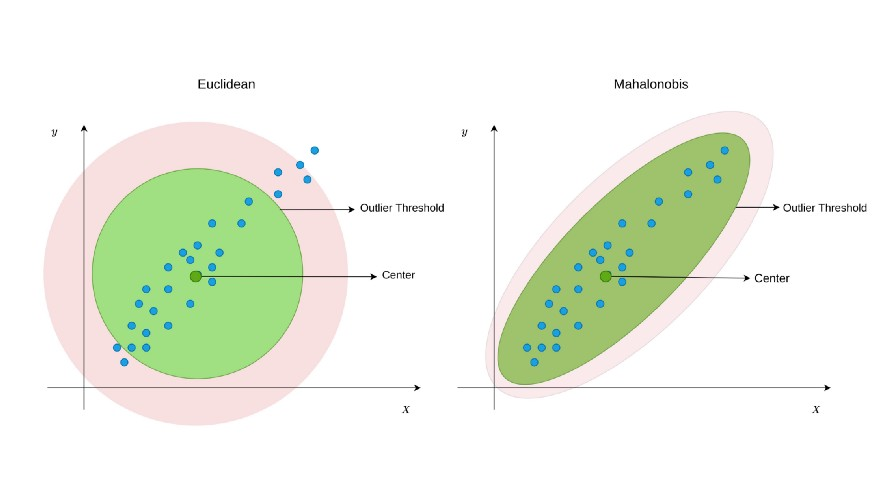
\includegraphics[width=.85\textwidth]{images/euclidean_vs_mahalanobis.jpeg}
		\captionof{figure}{Euclidean distance vs Mahalonobis distance, image by \cite{mahalanobis_medium}}
		\label{fig:6}
	\end{figure}
	
	Given a point $\va{x}=(x_1,x_2,...,x_N)^T$ extracted from a distribution of $m$ points in $\va{X}=(X_1,X_2,...,X_N)^T$ where $X_1,X_2,...,X_N$ are the random variables of the dataset; given $\va{\mu}=(\mu_1,\mu_2,...,\mu_N)^T$ the mean of the set of observations whose entries $\mu_i=\frac{1}{m}\sum{x_i}$, and the covariance matrix $\Sigma$ whose entry \begin{equation} \label{covariance_matrix}
\Sigma_{(i,j)}=cov[X_i,X_j]=E[(X_i-E[X_i])(X_j-E[X_j])]
	\end{equation}
	thus, the Mahalanobis Distance from a point $\va{x}$ and the set of points it has been extracted from is
	\begin{equation}
	d_M(\va{x},\va{\mu})=\sqrt{(\va{x}-\va{\mu})^T\Sigma^{-1}(\va{x}-\va{\mu})}
	\end{equation}
	The covariance matrix (equation \ref{covariance_matrix}) is estimated using the \texttt{numpy.cov} function, see the documentation \cite{numpy.cov} and the code for better understanding.\\
	\begin{figure}
		\centering
	\begin{minipage}[c]{0.45\textwidth}
			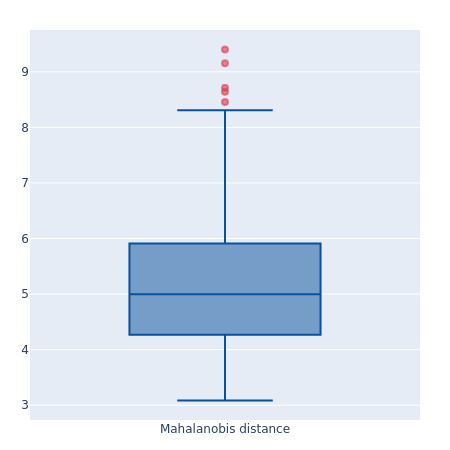
\includegraphics[width=\textwidth]{images/mahalanobis.png}
			\captionof{figure}{Box plot of Mahalonobis distance distribution}
			\label{fig:7}
	\end{minipage}
	\begin{minipage}{0.05\textwidth}
		\quad
	\end{minipage}
	\begin{minipage}[c]{0.45\textwidth}
			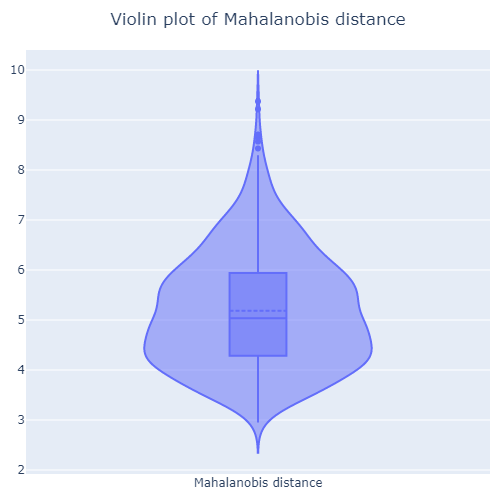
\includegraphics[width=\textwidth]{images/mahalanobis_violin.png}
			\captionof{figure}{Violin plot of Mahalonobis distance distribution}
			\label{fig:8}
	\end{minipage}
	\end{figure}
	Once computed the Mahalanobis distance for every point, its distribution can be evaluated to detect multidimensional outliers. As can be seen in figures [\ref{fig:7}] and [\ref{fig:8}], there are a few points (seven) whose distance is greater than $Q_3+1.5\cdot Q_3$, thus they could be considered as multidimensional outliers. However, they are a very small number of points and, among those, four have class label \texttt{0} (\texttt{bad} credit risk), that is the one with the lowest number of observations. That means that they could seem outliers because there are not so many samples of this label (considering that the ones present have already been oversampled), thus they could be significant points in detecting bad credit risk. In addition, all those points fall in the range of the so called \emph{suspected outliers}, while there are no points $< 4\cdot Q_1 - 3\cdot Q_3$ or $> 4\cdot Q_3 - 3\cdot Q_1$ (that are the ranges where points are very likely to be outliers). For these reasons, those seven points are not removed from the dataset.
	
	\subsection{Data normalization}
	When performing analysis with datasets whose features have different scales, data normalization is a very important step in the preprocessing procedure. Indeed, especially when applying some specific techniques that rely on distance or variance (e.g. distance-based classification algorithm, PCA and so on), if features are not rescaled, the distance between points and data variance are more affected by those features that have larger scale or higher values. Thus, the features end up not to have the same importance.\\
	In addition, although some algorithms' implementations take care of centering data (e.g. \texttt{sklearn.decomposition\\.PCA}\footnote{documentation at: \url{https://scikit-learn.org/stable/modules/generated/sklearn.decomposition.PCA.html}}), others do not (e.g. \texttt{sklearn.decomposition.KernelPCA}), thus in order to avoid problems in data analysis, data points are also centred.\\
	Specifically, the following transformation has been applied to features, that is, for each feature $X$, the new one $\hat{X}$:
	\begin{equation}
		\hat{X} = \frac{X - mean(X)}{max(X) - min(X)}
	\end{equation} 
	in this way, every feature is centered ($\mu_i = 0$) and rescaled in a unitary range. 
	
	\begin{figure}
		\centering
		\begin{minipage}[c]{0.40\textwidth}
			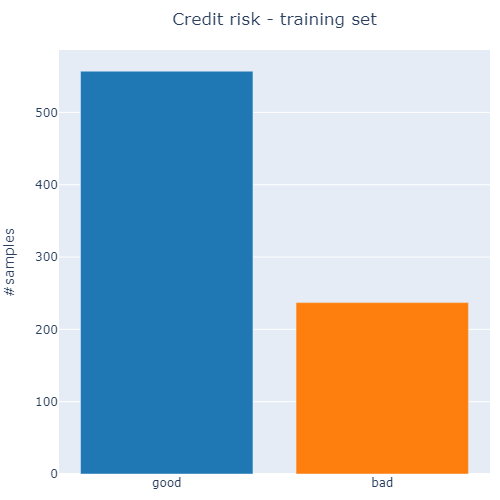
\includegraphics[width=\textwidth]{images/training_set.png}
			\captionof{figure}{Training set}
			\label{fig:9}
		\end{minipage}
		\begin{minipage}{0.05\textwidth}
			\quad
		\end{minipage}
		\begin{minipage}[c]{0.40\textwidth}
			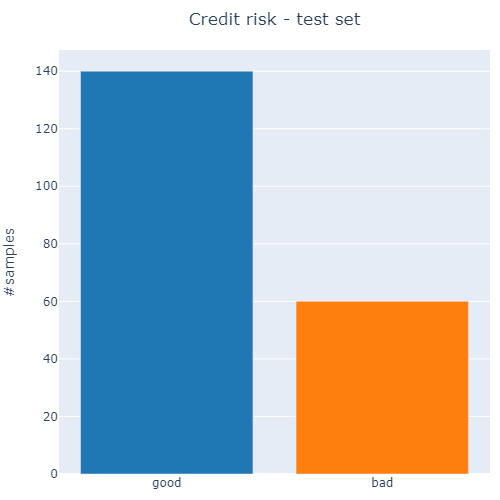
\includegraphics[width=\textwidth]{images/test_set.png}
			\captionof{figure}{Test set}
			\label{fig:10}
		\end{minipage}
	\end{figure}
	
	\subsection{Training-test split}
	To proceed in the classification phase, the dataset has been split into training and test set respectively for $80\%$ and $20\%$ in a stratified way, that means that in both sets, the proportion of \texttt{good} and \texttt{bad} credit risk of the original dataset has been kept [Figure \ref{fig:9} and \ref{fig:10}]. This is particularly important, because the test set (the one on which the trained classification algorithm will be evaluated), should be as much similar as possible to real data, that means keeping the proportion of label distribution, do not applying any further transformation to those data and do not use them during training. Indeed, all the dimensionality reduction techniques presented in the next section (\ref{dim_reduction}) has been applied only using the training set.
	
	\section{Dimensionality reduction} \label{dim_reduction}
	\subsection{Curse of dimensionality}
	After the encoding phase, the number of features (label excluded) went from 20 to 31. Of course, the encoding was needed, but in data analysis having to deal with many features can be problematic for a lot of reasons. Indeed this is called \emph{the curse of dimensionality}. When the dimensions increase, the volume of the hypercube containing the data increases as well, so all the points become more distant between them, thus making the dataset very sparse. To overcome this problem, the number of data points should increase exponentially with the dimension. Basically, all points become distant and at the same time they have similar distances among them; therefore, the concepts of nearest neighbours and distance become pointless. So, in cases like this, it is always a good idea to consider using a dimensionality reduction technique. 
	\subsection{Correlation based}
	One first intuitive way to reduce dimensionality is by looking at the pairwise correlation between features, in order to spot possible duplicated ones. In this case [Figure \ref{fig:12}], most of the features are almost not correlated, or with very low values of pairwise correlation. There are some higher values between the features that are the result of label encoding (especially \textbf{other\_installment\_plans} and \textbf{housing}). Indeed, those features are naturally correlated by construction and, as a matter of fact, their correlation is negative, since their values are all $0$s and $1$s, and if one of them has a $0$ there will be for sure another one having $1$ for that data point. This, together with the fact that each original feature has been encoded in a few number of new ones (from $2$ to $4$) and that in some cases their values were highly imbalanced, contribute to their correlation values. 
	\par In addition, it can be interesting to notice that there is a positive correlation ($\approx 0.65$) between \textbf{amount} and \textbf{duration} that can be explained by the fact that generally it needs more time to pay an higher credit, and between \textbf{property} and \textbf{housing\_3} ($\approx 0.52$), since the latter is $1$ when the person has its own house, and of course this feature's meaning partially overlaps with the other one.
	\par In any case, there are not situations where some features can be considered duplicated. Also by looking at the dendrogram [Figure \ref{fig:13}] (built by hierarchically clustering the pairwise features' distances using the average linkage), it can be seen that even the nearest features are quite distant among them.  
	
	%TODO dire che ho provato anche l'indice di spearman ma che ha prodotto risultati simili. è visibile sul sito/repo
	\begin{figure}[h]
		\centering
		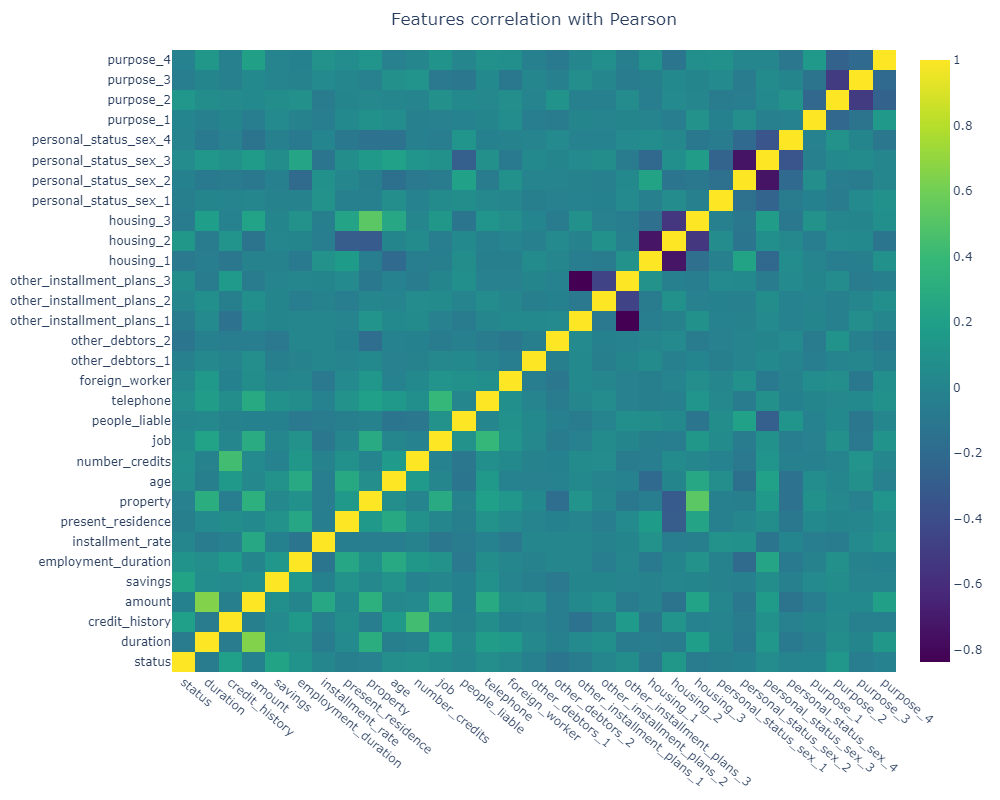
\includegraphics[width=.85\textwidth]{images/correlation_pearson.png}
		\captionof{figure}{Pairwise correlation according to Pearson coefficient }
		\label{fig:12}
	\end{figure}
	\begin{figure}[h]
		\centering
		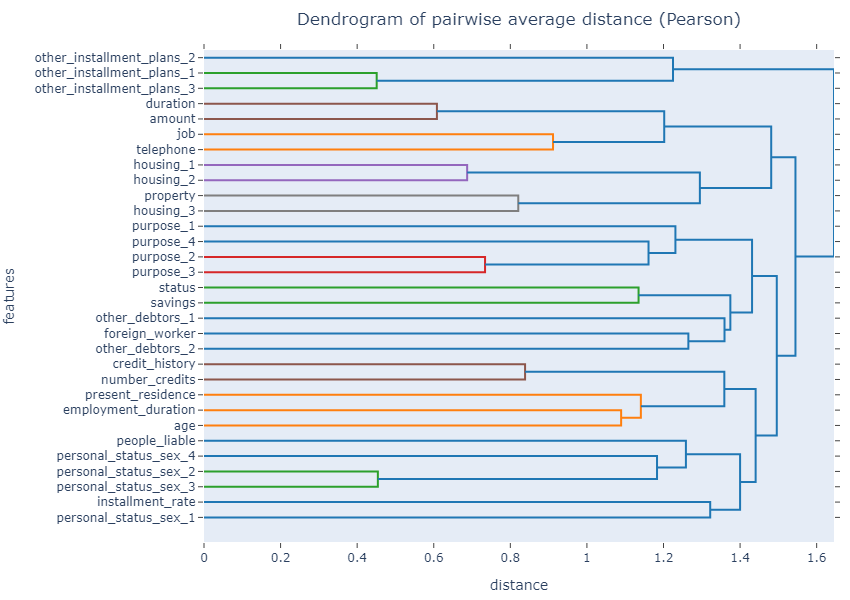
\includegraphics[width=.85\textwidth]{images/dendrogram_pearson.png}
		\captionof{figure}{Dendrogram of pairwise distance between features}
		\label{fig:13}
	\end{figure}
	
	\subsection{PCA}
	Principal Component Analysis is one of the most popular and simple techniques of dimensionality reduction. Its goal is to find a linear mapping that project the $m$ data points in a low dimensional space, from $d$ features to $n$, with $n << d$, in such a way that the information lost is as small as possible. 
	\begin{figure}[h]
		\centering
		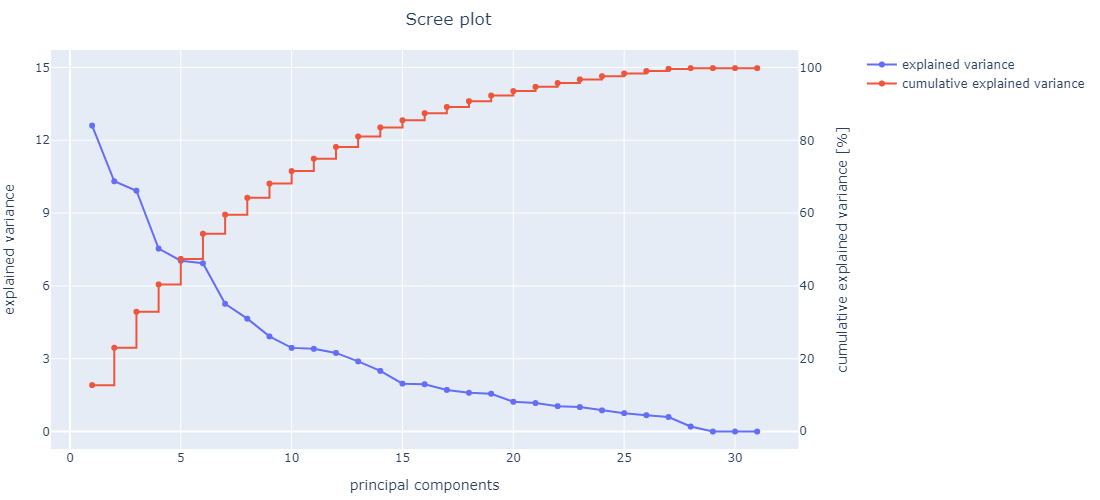
\includegraphics[width=.95\textwidth]{images/scree_plot.png}
		\captionof{figure}{Scree plot of principal components}
		\label{fig:11}
	\end{figure}
	This technique has two formulations that lead to the same solution from different points of view.
	\begin{itemize}
		\item the \textbf{minimum error} formulation, that finds a solution to the problem
		\begin{equation}
\underset{U\in \mathbb{R}^{n,d}}{\mathrm{argmin}}\, \sum_{i}^{m}\norm{\va{x}_i - UU^T\va{x}_i}^2_2 \quad \mathrm{subject\ to\ } U^TU=\mathbb{I}
		\end{equation}
	The idea is that we want minimise the error, that is the information we loose, in projecting the data in a lower dimensional space. Indeed, the error is computed between each original point $\va{x}$ and its reconstruction $\hat{\va{x}}=UU^T\va{x}$. \\
	Assuming that the data points are centered ($\va{\mu}=\va{0})$, and given the matrix of data points $X \in \mathbb{R}^{m,d}$, $m$ number of points and $d$ number of features, the solution to find the linear mapping (the orthogonal matrix $U^T$) is finding the $n$ eigenvectors ($\va{u}_1,\va{u}_2,...,\va{u}_n$) corresponding to the $n$ biggest eigenvalues ($\lambda_1\ge \lambda_2\ge ... \ge \lambda_n \ge ... \ge \lambda_d$) of the covariance matrix of $X$. Those eigenvectors (the \emph{principal components}) are the column of the matrix $U$, and the sum of the remaining eigenvalues is the error done in projecting the data in low dimensional space. However, since the data distribution is not known, the covariance matrix is estimated through the scatter matrix, also called sample covariance matrix
	\begin{equation} \label{scatter_matrix}
		S = X^TX
	\end{equation}
	still assuming $\va{\mu}=\va{0}$.
	\item the \textbf{maximum variance} formulation, that aims to find as principal components the directions where the variance of the projection of data points is maximized, since the idea is that the directions where the variance is maximum, are the ones where the information carried also is maximal. Those directions are to be found one at a time, and for each one the variance of data along that direction should be maximized,  enforcing the constraints that each principal component must have norm $1$ and it has to be orthogonal with respect to the previous ones. \\
	In the end, it turns out that finding the first n principal components $\va{u}_1,\va{u}_2,...,\va{u}_n$ means to find the $n$ eigenvectors of the sample covariance matrix (equation \ref{scatter_matrix}) and that their corresponding eigenvalues, are exactly the variance of the points projected along that directions. In particular, the first $n$ eigenvectors found with the maximization variance method, are the ones corresponding to the $n$ maximum eigenvalues of the matrix $S$. Thus, the two methods are exactly equivalent.
	\end{itemize}
	\par In order to decide how many principal components to take, a trade off must be found in order to take neither too little information, nor too many features. 
	Here [Figure \ref{fig:11}] both the explained variance (the eigenvalues drown in descending order) and the cumulative explained variance (for each eigenvalue, its ratio w.r.t. the sum of all eigenvalues is computed, then drown in a cumulative way) are showed. In this case, since there is an elbow at $15$ principal components, and since at that point the cumulative explained variance is sightly higher than $85\%$, I decided to take $15$ as number of principal components to keep.

	\subsection{Kernel PCA} 	
	A possible variation of the above technique is its Kernel extension. In fact, the Kernel PCA does the same as PCA, but it operates in a high dimensional space. The idea behind this relies on the intuition that many datasets, which are not linearly separable in their space, can be made linearly separable by projecting them into a higher dimensional space; then, in that space, PCA is more likely to give a good result.\\ However, assuming that a mapping $\Phi$ from the feature space to a Reproducing Kernel Hilbert Space (RKHS) exists, there is no need to map all points $\va{x} \rightarrow \Phi(\va{x})$ and apply PCA on the new space. Indeed, thanks to the \emph{Mercer's theorem}, we only need a symmetric function $k: \raisebox{2pt}{$\chi$} \times \raisebox{2pt}{$\chi$} \rightarrow \mathbb{R}$ positive semi-definite to have the assurance that $k$ implements an inner product in some RKHS; thus, there is no need neither to compute $\Phi$, nor to project the data points in the Hilbert space. Specifically, given $n$ data points ($\va{x}_i$) and the matrix $K_{n\times n}$ whose element $K(i,j)=\Phi(\va{x}_i)^T\cdot\Phi(\va{x}_j)=k(\va{x}_i,\va{x}_j)$, the KPCA solution is just finding the top $d$ eigenvectors of $K$, corresponding to the highest eigenvalues. \\
	In particular, in the implementation by \texttt{sklearn}\footnote{documentation at: \url{https://scikit-learn.org/stable/modules/generated/sklearn.decomposition.KernelPCA.html}}, there are four possible non-linear kernels: poly, rbf, sigmoid and cosine.
	\begin{figure}[h]
		\centering
		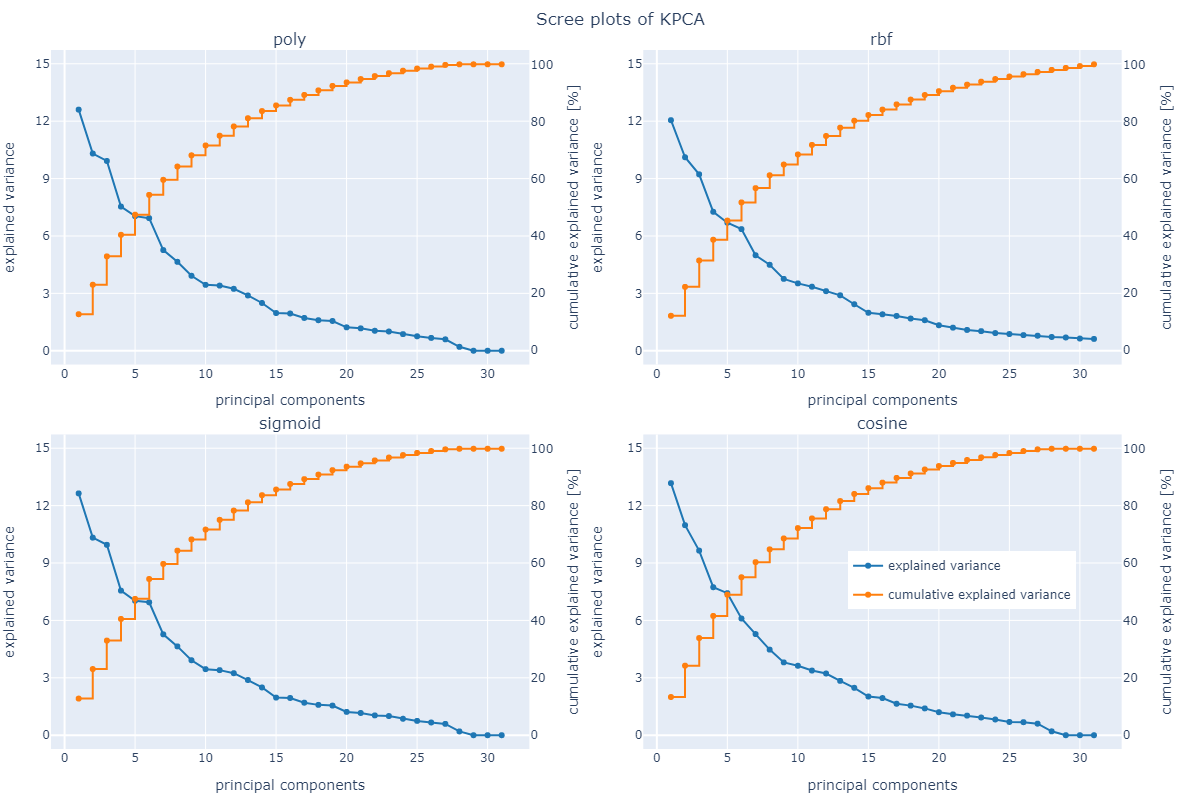
\includegraphics[width=.9\textwidth]{images/scree_plot_kpca.png}
		\captionof{figure}{Scree plot of KPCA with four different kernels}
		\label{fig:14}
	\end{figure}
	To compare those kernels, a grid search (5-fold cross validation, the default one for \texttt{sklearn.model\_selection\\.GridSearchCV}\footnote{documentation at: \url{https://scikit-learn.org/stable/modules/generated/sklearn.model_selection.GridSearchCV.html}} function) has been performed for each one to choose the best hyperparameters that minimize the mean squared error on the reconstruction of data points; in terms of this metric the best one seems to be \texttt{poly}, the polynomial kernel. However, by looking at their Scree plots [Figure \ref{fig:14}], they seem pretty similar both among them and with respect to the result of standard PCA [Figure \ref{fig:11}]: they all have an elbow in explained variance graph around $15$ principal components, and in that point the cumulative explained variance is around $85\%$ ($82\%$ for \texttt{rbf} kernel).
	
	\subsection{mRMR}
	\par Unfortunately, a downside of [Kernel] PCA, is that the resulting principal components, that will be the new features used in the classification algorithms, are no longer features with a specific meaning. Instead, they are mappings (linear or not) of the original ones, thus making the interpretability of the classification models very difficult. For this reason, it is interesting to explore methods of dimensionality reduction whose goal is to keep a limited number of the original variables with some specific criteria. For example, the algorithm written by Peng \emph{et al.}\cite{Peng05featureselection} operates an heuristic feature selection based on minimum Redundancy and Maximum Relevance (mRMR)\footnote{documentation at: \url{https://pypi.org/project/pymrmr/}}. Basically it tries to select features by minimizing the dependency among them and maximizing the mean of the mutual information between every feature and the class label. The authors of the paper have investigated two ways to combine redundancy and relevance: the Mutual Information Quotient (MIQ) and the Mutual Information Difference (MID); that is using respectively their ratio or their difference. To evaluate the classification results of this method with the others, it has been set to select $15$ features, that for the two schemas are respectively:
	\begin{itemize}
		\item \textbf{MIQ}: status, foreign\_worker, other\_installment\_plans\_2, purpose\_2, credit\_history, property, savings, housing\_1, personal\_status\_sex\_1, other\_installment\_plans\_1, other\_debtors\_1, other\_debtors\_2, age, number\_credits, installment\_rate,
		\item \textbf{MID}: status, foreign\_worker, credit\_history, purpose\_2, savings, housing\_2, other\_installment\_plans\_3, personal\_status\_sex\_1, other\_debtors\_1, amount, duration, number\_credits, other\_debtors\_2, age, installment\_rate
	\end{itemize}
	As can be seen, most of the features selected with the two methods are the same.
	\section{Cross validation pipeline} \label{cv}
	At this point, the classification models can be trained to be able to detect good and bad creditors. However, each model can depend on one or more hyperparameters, that are the parameters that control the training process in the machine learning algorithm. In order to choose the best values that make the models to outperform in the desired task, a cross validation process is needed. \\
	First of all, $5$ different training sets are prepared, one for each dimensionality reduction technique discussed above (Section \ref{dim_reduction}): PCA, KernelPCA, mRMR with method MIQ and mRMR with method MID, plus the one without dimensionality reduction.\\
	Then, for each of those training sets, a stratified $10$-fold cross validation (\texttt{GridSearchCV}\footnote{documentation at: \url{https://scikit-learn.org/stable/modules/generated/sklearn.model_selection.GridSearchCV.html}} function of \texttt{sklearn} library) is run for each combination of dataset balancing technique (Section \ref{dataset_balancing}) and classification algorithm (Section \ref{classification}) in order to find the best classification pipeline. 
	In particular, a few comments are necessary:
	\begin{itemize}
		\item the $10$-fold has to be stratified because at each step the validation fold, used to test performances, must have the same characteristics of the test set;
		\item for the same reason, the dataset balancing technique is applied only to the $9$ folds used for training;
		\item unfortunately, the same was not possible for the dimensionality reduction techniques, since the mRMR method has not been implemented to be part of a pipeline, thus they have all been applied to the entire training set (but not to the test set). Assuming that the $10$ fold are sampled in a random way, at each step the $10^{th}$ one should not have such different characteristics with respect to the the other ones;
		\item using a k-fold cross validation instead of the classical train-validation split of the training set, is helpful in trying to reduce overfitting.
	\end{itemize}
	Given the following metrics
	\begin{itemize}
		\item $\mathrm{accuracy} = \frac{\mathrm{TP}+\mathrm{TN}}{\mathrm{TP}+\mathrm{FP}+\mathrm{TN}+\mathrm{FN}}$
		\item $\mathrm{precision} = \frac{\mathrm{TP}}{\mathrm{TP}+\mathrm{FP}}$ 
		\item $\mathrm{recall} =  \frac{\mathrm{TP}}{\mathrm{TP}+\mathrm{FN}}$
		\item $\mathrm{F1} = 2 * \frac{\mathrm{precision}*\mathrm{recall}}{\mathrm{precis	ion}+\mathrm{recall}}$
	\end{itemize}
	where TP (\emph{True Positive}), FP (\emph{False Positive}), TN (\emph{True Negative}) and FN (\emph{False Negative}) are respectively \texttt{bad} credit risk correctly classified, \texttt{good} credit risk wrongly classified, \texttt{good} credit risk correctly classified and \texttt{bad} credit risk wrongly classified. \\
	In the cross validation step, the chosen metric to be maximized is the F1 score.
	It is probably the best score for this kind of problems, because the accuracy may not be the good choice when dealing with an imbalanced dataset, since it just counts the correctly classified points with respect to all the points, without taking into account the label imbalance. The F1 score, instead, enforces the models to correctly classify the minority class points.

	\section{Dataset balancing} \label{dataset_balancing}
	Dealing with a dataset where the class labels' distribution is imbalanced [Figure \ref{fig:1}] may lead to poor performing classification algorithms, because most of them assume that class labels are equally distributed and that an be problematic mostly in cases like this one, where we are more interested in detecting the minority class than the majority one: we want the algorithms to be able to properly detect the bad creditors.\\
	For this reason, three main techniques have been investigated: oversampling, undersampling and SMOTE.
	\subsection{Undersampling}
	With this technique, given a training set with $N$ points in the minority class and $M$ in the majority one ($M > N$), in order to balance the class labels' distribution, $N$ points are randomly sampled from the majority class. The main downside is that we are removing samples from the original dataset, possibly taking away useful information to correctly classify data.
	\subsection{Oversampling}
	This technique aims to reach a uniform distribution in class labels by randomly sampling data from the minority class, until its number of samples matches the one of the majority class. Of course there is no longer the problem of loosing information, however, given the big gap between the two labels, overfitting is more likely to occur. Especially with this dataset, whose minority class has already been oversampled from $5\%$ to $30\%$ as reported by Grömping \cite{gromping}.
	\subsection{SMOTE}
	Synthetic Minority Oversampling Technique (SMOTE) is again an oversampling technique, but instead of randomly sampling points from the minority class, they are linearly combined to synthetically generate new points. In order to augment data, for each data point in the minority class, its k-nearest neighbours (e.g. k$=5$) are found and, among them, one is randomly selected. The new point is generated as a convex combination of the two data points. \\
	Although this can be a good way to balance the dataset without incurring in overfitting, it is designed to work only with continuous data. Indeed categorical features, even if properly encoded, have a fixed and limited amount of possible values; thus, it is likely that synthetically generated points would have inconsistent values. 
	
	\section{Classification models} \label{classification}
	In this section, all the classification models trained with this dataset are investigated. As mentioned before, a $10$-fold cross validation is run to decide the best dimensionality reduction technique, balancing technique as well as the models' hyperparameters. 
	\subsection{Decision Tree}
	\begin{figure}[h]
		\centering
		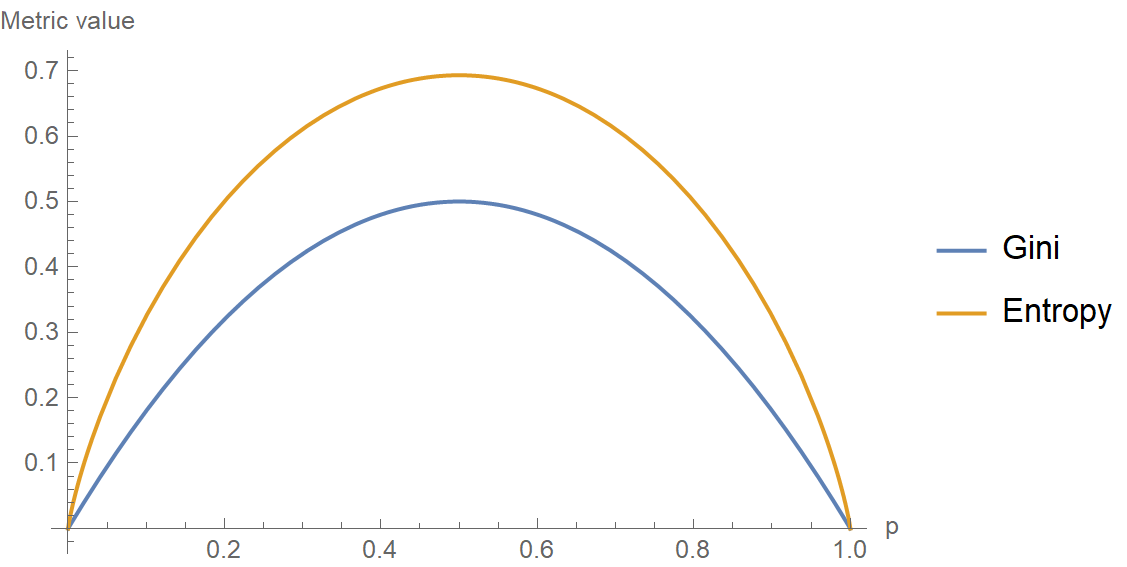
\includegraphics[width=.55\textwidth]{images/gini_vs_entropy.png}
		\captionof{figure}{Gini index compared to cross-entropy. Image by \cite{ginivsentropy}}
		\label{fig:15}
	\end{figure}
	Decision tree is a very popular tool used both for classification and regression. At the basis, the idea is to divide the predictor space into $N$ non overlapping regions where the assumption is that in every region only one label is assigned, such that the prediction error is minimized with the lowest number of regions. Unfortunately, this procedure is computationally unfeasible, because the minimum amount of regions involved in the minimization process is equal to the number of training points. Thus, decision trees are built with a top-down greedy procedure, where at each step the best current split is done and so on until in each region there is only one label. To decide which one is the best, a criterion must be used, either the \emph{Gini index} (eq \ref{gini}), a measure of node purity that assumes small values when a node contains more observations of the same class, or the \emph{cross-entropy} (eq \ref{entropy}), very similar to the previous one, but it tends to penalize less small impurities, since it assumes lower values with respect to \emph{Gini} [Figure \ref{fig:15}]; here it is treated as an hyperparameter of the model (\texttt{criterion}). \\
	Given $K$ the number of classes (here 2), $m$ the current split (or region) and $\hat{p}_{mk}$ the proportion of the points from the $k^{th}$ in the $m^{th}$ region:
	\begin{equation} \label{gini}
		\mathrm{Gini\ index}=\sum_{k=1}^{K}\hat{p}_{mk}(1-\hat{p}_{mk})
	\end{equation}
	\begin{equation} \label{entropy}
		\mathrm{Cross\mbox{-}entropy}=\sum_{k=1}^{K}\hat{p}_{mk}\log\hat{p}_{mk}
	\end{equation}\\
	However, the main disadvantage of this model is that it is prone to overfitting. Indeed, if the tree is built until no further split can be done, the model ends up describing the training set itself without a predicting goal. For this reason, two main strategies have been applied:
	\begin{itemize}
		\item one way is to set some hyperparameters of the problem to limit this phenomena, such as the depth of the tree (\texttt{max\_depth}), the minimum number of samples in leaves (\texttt{min\_samples\_leaf}) or the minimum number of samples to split a node (\texttt{min\_samples\_split}). They can be expressed both in absolute values or as a fraction of the whole training set.
		\item another way is to do the other way around: the tree is firstly built until every split can be done, then it is pruned by progressively substituting subtrees with leaves. The objective is to minimize the error function as before, but it now has a regularization term that consists in the number of leaves of the node weighted for an hyperparameter $\alpha$ (\texttt{ccp\_alpha}).
	\end{itemize}
	
	\subsection{Tree-based ensemble methods}
	Another way to overcome overfitting and variance and improve generalization of decision tree classifier, is by applying an ensemble method. The idea is that combining multiple weak models (trees in this case) can improve results with respect to keeping a single model. In classification, the final prediction of a new point is the majority of the models' predictions. Here two procedures are taken into account. In both cases, they have been cross-validated and then trained with the strategies discussed above (with and without pruning); however to perform a fair comparison, decision tree hyperparameters have not been tuned again, but the ones previously obtained (best result with undersampling and best result with oversampling) are used.
	\subsubsection{Bagging}
	With this method, $B$ sets of point are generated by taking samples (with repetition) from the original training set (this procedure is called \emph{Bootstrap}), then from each one a tree is built as explained before. The tuned hyperparameters are: the number of samples of each set of point (\texttt{max\_samples}) expressed as the percentage of the training set, and the number of estimators (\texttt{n\_estimators}), that is also the number of sets $B$.
	\subsubsection{Random Forest}
	Random forest, instead, is an improvement of bagging. Indeed, it builds decision trees on bootstrapped training samples, but in addition, each time a split has to be done in the tree building procedure, only a limited and random selection of features is considered. Here only the number of trees in the random forest is tuned (\texttt{n\_estimators}).
	\subsection{Logistic Regression}
	Logistic regression is a classification method based on the composition of the sigmoid function $\sigma$ and the class of linear functions. Thus, the hypothesis classifier is 
	\begin{equation}
		H = \{ \vec{x}\mapsto \sigma(\langle\vec{x},\vec{\beta}\rangle) : \vec{\beta}\in\mathbb{R}^d\}
	\end{equation}
	Where $H(\vec{x})$ is a real value in the interval $(0,1)$ and it corresponds to the probability of the point $\vec{x}$ to have label $y = 1$ (viceversa, the probability to have label $y=0$ is $1-H(\vec{x})$). However, since in classification we want the model to predict a label, a threshold is needed to decide whether the outcome is label $0$ or $1$. \\
	In this model, the hyperparameters to be tuned involve the regularization term used in parameters' optimization, whose role is to avoid overfitting and simplify the model itself. Here two kind of regularizations are considered (via the \texttt{penalty} hyperparameter): the Ridge regression ($\lambda\lVert{\vec{\beta}}\rVert^2_2$), or the LASSO one ($\lambda\lVert{\vec{\beta}}\rVert_1$), where $\lambda = \frac{1}{C}$ (\texttt{C} is the other hyperparameter tuned in cross-validation).
	\subsection{Support Vector Machine} \label{svm}
	Support Vector Machine (SVM) is a supervised learning model used for regression and classification, specifically, it is particularly useful for binary classification. Indeed, its goal is to find an hyperplane separating points of the two classes in the best way possible. This can be done by maximizing the margin (\emph{Hard margin SVM}), that is the minimal distance of the hyperplane with the data points. However it is feasible only if the samples are linearly separable, which is a very unrealistic assumption. Therefore, a more realistic approach is used (\emph{Soft margin SVM}) that still aims to find the best hyperplane, but allowing the model to make some mistakes. Eventually the problem becomes:
	\begin{equation}
		\underset{\vec{w}, b}{\mathrm{argmin}}\, \frac{1}{2}\lVert\vec{w}\rVert_2^2 + C\sum_{i}\xi_i \quad \mathrm{subject\ to\ }y_i[\langle \vec{w},\vec{x}\rangle+b]\ge1-\xi_i \mathrm{\ and\ } \xi_i\ge0
	\end{equation}
	where $\langle\vec{w},\vec{x}\rangle+b = 0$ is the hyperplane separating data points $(\vec{x}_i,y_i)$, and $\xi_i$ are the so called slack variables that are introduced to loosen the assumption of linear separability, weighted for the hyperparameter \texttt{C}.\\
	As previously done in Kernel PCA, also SVM can be used with kernels, that means applying SVM in an higher dimensional space where points are more likely to be linearly separable, to find eventually an hypercurve separating points in feature space. This is possible because of the dual formulation of SVM that reduces the problem to:
	\begin{equation}
		\underset{\vec{\alpha}}{\mathrm{argmax}}\, -\frac{1}{2}\sum_{i,j}\alpha_i\alpha_jy_iy_j\langle\vec{x_i},\vec{x_j}\rangle + \sum_{i}\alpha_i \quad \mathrm{subject\ to\ } \sum_{i}\alpha_iy_i=0 \mathrm{\ and\ } \alpha_i\in[0,C]
	\end{equation}
	where the scalar product $\langle\vec{x_i},\vec{x_j}\rangle$ can be easily substituted with $k(x_i,x_j)$, being $k$ the kernel function that represents the inner product in an higher dimensional Hilbert space. \\
	As in KPCA, the possible values for \texttt{kernel} parameter are:
	\begin{itemize}
		\item \texttt{linear}: no kernel is used, it is simply the scalar product $\langle\vec{x_i},\vec{x_j}\rangle$
		\item \texttt{poly}: the polynomial kernel $(\gamma\langle\vec{x_i},\vec{x_j}\rangle+r)^d$
		\item \texttt{rbf}: the radial basis function kernel $e^{-\gamma\lVert x_i+x_j\rVert^2}$
		\item \texttt{sigmoid}: $\tanh(\gamma\langle\vec{x_i},\vec{x_j}\rangle+r)$
	\end{itemize}
	where $\gamma$ (\texttt{gamma}), $r$ (\texttt{coef0}) and $d$ (\texttt{degree}), together with the kind of \texttt{kernel} and \texttt{C} are the hyperparameters to be tuned.\\
	Due to computational reasons, this model's hyperparameters has been tuned with a $2$-fold cross validation; indeed every combination (dimensionality reduction method, balancing dataset method) requires at least $1$ hour and at least $1/2$ hour respectively with $10$-fold and $5$-fold cross validation.
	
	\subsection{K-Nearest Neighbours}
	K-Nearest Neighbours is a very simple classification and regression supervised model. Basically, when a new point has to be classified, it is assigned to the most common class (in case of classification) among $k$ nearest points in the training set; while in case of regression, the average of the $k$ neighbours' values is computed. \\ 
	$k$ (\texttt{n\_neighbors}) is of course the most important hyperparameter to tune, and it is chosen among the odd values, since in binary classification this ensures that only one label will have the maximum number of votes. Then, the other tuned hyperparameters are:
	\begin{itemize}
		\item \texttt{p}, that is the power parameter of the Minkowski distance metric $(\sum_{i}^{d}| x_i- y_i|^p)^{1/p}$, being $d$ the number of features and $\vec{x}$ and $\vec{y}$ the points among which the distance is to be computed. For instance $p=1$ is the Manhattan distance, and $p=2$ is the Euclidean distance;
		\item \texttt{weights}, by which it is possible to weight the votes basing on point's inverse of distance, in order to weight more nearest points with respect to far ones.
	\end{itemize}
	It is a completely data-driven model, since it does not require any training and its prediction strictly depends on training data; however, it might take longer with respect to other models to give a prediction, and it requires a significant amount of memory to keep all training points.
	\subsection{Fisher Discriminant Analysis}
	With the actual dataset, Linear Discriminant Analysis (LDA) and Quadratic Discriminant Analysis (QDA) can not be applied. They both aim to find a combination of features (linear or quadratic) with the goal to separate classes. However, the assumption for both is the multivariate normality, that means that each feature of the dataset should be normally distributed. It can be clearly seen from Figure \ref{fig:2} that this is not the case. Furthermore, a Henze-Zirkler Multivariate Normality Test (\texttt{multivariate\_normality} from the \texttt{pingouin} library\footnote{documentation at \url{https://pingouin-stats.org/generated/pingouin.multivariate_normality.html}}) has been performed: it returns the \emph{p-value} related to the null hypothesis that the variables follow a multivariate normal distribution, in this case it is much lower than the default threshold $\alpha = 0.05$, that means that the null hypothesis is rejected.
	\par On the other hand, the Fisher Discriminant Analysis, that actually is a special case of LDA, do not impose any assumption on data distribution. Its goal is to find a lower dimensional space where points are linearly separable, thus they can be better classified. The idea has some similarities with PCA, indeed FDA tries to find a space $V$ where the projected data points have maximum distance among the class means and the minimum class variances. Practically the problem becomes 
	\begin{equation}
		\underset{V}{\mathrm{argmax}}\, \frac{det(V^TS_BV)}{det(V^TS_WV)}
	\end{equation}
	being $S_B$ and $S_W$ the matrices measuring respectively the separation between the means of classes before projection and the sum of the class scatter matrices. Eventually it turns to be finding the eigenvectors of matrix $S_W^{-1}S_B$ that are at most $c-1$, where $c$ is the number of classes.
	Unlike PCA, this method is supervised and has a limitation on the lower dimensional space' dimension.
	\\ This technique has not been implemented by \texttt{sklearn} library, but an implementation from Kawin Nikomborirak\footnote{documentation at: \url{https://pypi.org/project/kfda/}} is distributed in \texttt{kfda} library, based on Ghojogh \emph{et al.} paper \cite{ghojogh2019fisher}. This library offers also the kernel extension of FDA algorithm, and uses \texttt{scikit-learn} interface, thus giving the possibility to use the same methods. Since the number of components of the lower dimensional space is fixed to $1 = c-1$, the hyperparameter to be tuned is only the \texttt{kernel} type; unfortunately, kernel's parameters can not be tuned easily with the actual implementation of this function, thus the default ones provided by \texttt{sklearn} are used.

	\section{Classification results}
	In this section, the results of the above algorithm are presented. They are trained on the whole training set with the tuned hyperparameters, and then evaluated on the test set. The metrics used to evaluate performances are the ones already mentioned in Section \ref{cv}: \emph{accuracy}, \emph{precision}, \emph{recall} and \emph{F1}. The \emph{confusion matrix} is also used to better visualize results.
	\begin{figure}[!ht]
	\centering
		\begin{minipage}[t]{0.45\textwidth}
			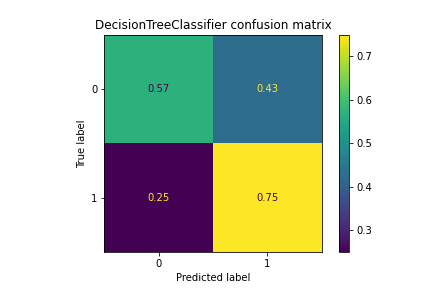
\includegraphics[width=.85\textwidth]{images/confusion_DecisionTreeClassifier.png}
			\setlength{\belowcaptionskip}{-5pt}
			\captionof{figure}{Decision Tree; no dimensionality reduction, oversampling and hyperparameters \texttt{max\_depth}=$6$, \texttt{criterion}=\emph{gini}, \texttt{min\_samples\_split}=$0.45$ and \texttt{min\_samples\_leaf}=$0.001$}
			\label{fig:16}
		\end{minipage}
		\begin{minipage}{0.05\textwidth}
			\quad
		\end{minipage}
		\begin{minipage}[t]{0.45\textwidth}
			
\includegraphics[width=.85\textwidth]{images/confusion_DecisionTreeClassifierWithPruning.png}
			\setlength{\belowcaptionskip}{-5pt}
			\captionof{figure}{Decision Tree With Pruning; no dimensionality reduction, oversampling and hyperparameters \texttt{criterion}=\emph{entropy} and \texttt{ccp\_alpha}=$0.02$}
			\label{fig:17}
		\end{minipage}
		\begin{minipage}[t]{0.45\textwidth}
			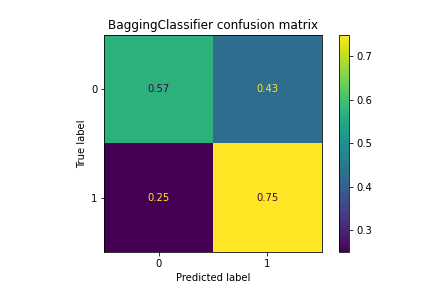
\includegraphics[width=.85\textwidth]{images/confusion_BaggingClassifier.png}
			\setlength{\belowcaptionskip}{-5pt}
			\captionof{figure}{Bagging; no dimensionality reduction, oversampling, [Figure \ref{fig:16}] hyperparameters and \texttt{n\_estimators}=$10$ and \texttt{max\_samples}=$0.75$}
			\label{fig:18}
		\end{minipage}
		\begin{minipage}{0.05\textwidth}
			\quad
		\end{minipage}
		\begin{minipage}[t]{0.45\textwidth}
			
\includegraphics[width=.85\textwidth]{images/confusion_BaggingClassifierWithPruning.png}
			\setlength{\belowcaptionskip}{-5pt}
			\captionof{figure}{Bagging With Pruning; no dimensionality reduction, oversampling, [Figure \ref{fig:17}] hyperparameters and \texttt{n\_estimators}=$1000$ and \texttt{max\_samples}=$0.25$}
			\label{fig:19}
		\end{minipage}
		\begin{minipage}[t]{0.45\textwidth}
			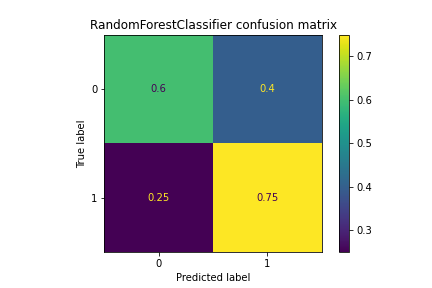
\includegraphics[width=.85\textwidth]{images/confusion_RandomForestClassifier.png}
			\setlength{\belowcaptionskip}{-10pt}
			\captionof{figure}{Random Forest; no dimensionality reduction, undersampling, hyperparameters of the best Decision Tree with undersampling and \texttt{n\_estimators}=$100$}
			\label{fig:20}
		\end{minipage}
		\begin{minipage}{0.05\textwidth}
			\quad
		\end{minipage}
		\begin{minipage}[t]{0.45\textwidth}
			
\includegraphics[width=.85\textwidth]{images/confusion_RandomForestClassifierWithPruning.png}
			\setlength{\belowcaptionskip}{-10pt}
			\captionof{figure}{Random Forest With Pruning; no dimensionality reduction, oversampling, [Figure \ref{fig:17}] hyperparameters and \texttt{n\_estimators}=$100$}
			\label{fig:21}
		\end{minipage}
	\end{figure}
	Surprisingly, for all classification algorithm, the best F1 scores during cross validation are obtained using the original training set without any dimensionality reduction technique applied. However, they only exceeded the other ones by a few percent, and generally all results were under $65\%$ of F1. Here [Figure \ref{fig:16}-\ref{fig:25}] the confusion matrices obtained from testing the best combination of dimensionality reduction, balancing technique and hyperparameters for each algorithm are shown.
	\begin{figure}[!ht]
		\centering
		\begin{minipage}[t]{0.45\textwidth}
			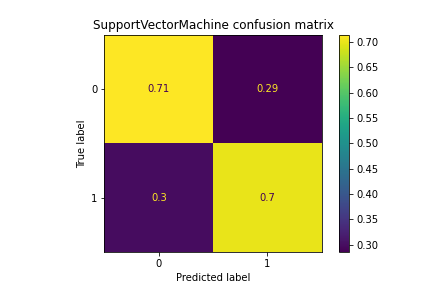
\includegraphics[width=.85\textwidth]{images/confusion_SupportVectorMachine.png}
			\setlength{\belowcaptionskip}{-5pt}
			\captionof{figure}{SVM; no dimensionality reduction, oversampling, hyperparameters \texttt{C}=$1$ and \texttt{kernel}=\emph{poly}, \texttt{gamma}=$0.01$, \texttt{coef0}=$1$ and \texttt{degree}=$5$}
			\label{fig:22}
		\end{minipage}
		\begin{minipage}{0.05\textwidth}
			\quad
		\end{minipage}
		\begin{minipage}[t]{0.45\textwidth}
			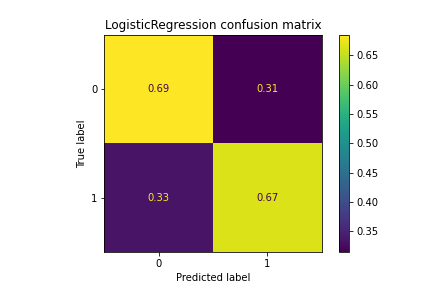
\includegraphics[width=.85\textwidth]{images/confusion_LogisticRegression.png}
			\setlength{\belowcaptionskip}{-5pt}
			\captionof{figure}{Logistic Regression; no dimensionality reduction, undersampling, hyperparameters \texttt{C}=$1$ and \texttt{penalty}=\emph{l2}}
			\label{fig:23}
		\end{minipage}
		\begin{minipage}[t]{0.45\textwidth}
			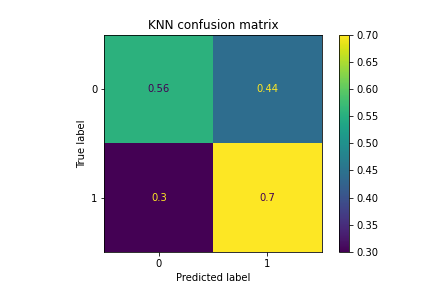
\includegraphics[width=.85\textwidth]{images/confusion_KNN.png}
			\captionof{figure}{K-Nearest Neighbors; no dimensionality reduction, undersampling, hyperparameters \texttt{n\_neighbors}=$13$, \texttt{p}=$1$, \texttt{weights}=\emph{distance}}
			\label{fig:24}
		\end{minipage}
		\begin{minipage}{0.05\textwidth}
			\quad
		\end{minipage}
		\begin{minipage}[t]{0.45\textwidth}
			
\includegraphics[width=.85\textwidth]{images/confusion_FisherDiscriminantAnalysis.png}
			\captionof{figure}{Fisher Discriminant Analysis; no dimensionality reduction, oversampling, and \texttt{kernel}=\emph{linear}}
			\label{fig:25}
		\end{minipage}
	\end{figure}
	\begin{table}[!ht]
		\centering
			\begin{tabular}{l|c|c|c|c|}
				&	\textbf{Accuracy}	& \textbf{Precision} &	\textbf{Recall	}&\textbf{F1}\\
				\hline
				\textbf{Decision Tree	}&0.685&	0.479&	0.583&	0.526\\
				\hline
				\textbf{Decision Tree With Pruning} &	0.650&	0.448&	0.717&	0.551\\
				\hline
				\textbf{Bagging }&	0.625&	0.429&	0.750&	0.545\\
				\hline
				\textbf{Bagging With Pruning}&	0.695&	0.494&	0.700&	0.579\\
				\hline
				\textbf{Random Forest }&	0.645&	0.446&	0.750&	0.559\\
				\hline
				\textbf{Random Forest With Pruning}&	0.655&	0.451&	0.683&	0.543\\
				\hline
				\textbf{Support Vector Machine}&	0.710&	0.512&	0.700&	0.592\\
				\hline
				\textbf{Logistic Regression}&	0.680&	0.476&	0.667&	0.556\\
				\hline
				\textbf{K-NN}&0.600&	0.404&	0.700&	0.512\\
				\hline
				\textbf{Fisher Discriminant Analysis}&	0.720&	0.525&	0.700&	0.600\\
				\hline
			\end{tabular}
			\caption{Evaluating metrics for all classification models' best pipelines and hyperparameters.}
	\end{table}

	\nocite{MohriRostamizadehTalwalkar18}
	\nocite{understandingml}
	\nocite{ghojogh2019fisher}
	% TODO use \nocite{key} to include in the references :
	% - libro da cui ho guardato la PCA ?
	\newpage
	\addcontentsline{toc}{section}{References}
	\printbibliography
	
	% TODO:
	% - scrivere le funzioni + documentazione usata per ogni modello (?)
	
\end{document}